% Options for packages loaded elsewhere
\PassOptionsToPackage{unicode}{hyperref}
\PassOptionsToPackage{hyphens}{url}
\PassOptionsToPackage{dvipsnames,svgnames,x11names}{xcolor}
%
\documentclass[
]{article}
\usepackage{amsmath,amssymb}
\usepackage{iftex}
\ifPDFTeX
  \usepackage[T1]{fontenc}
  \usepackage[utf8]{inputenc}
  \usepackage{textcomp} % provide euro and other symbols
\else % if luatex or xetex
  \usepackage{unicode-math} % this also loads fontspec
  \defaultfontfeatures{Scale=MatchLowercase}
  \defaultfontfeatures[\rmfamily]{Ligatures=TeX,Scale=1}
\fi
\usepackage{lmodern}
\ifPDFTeX\else
  % xetex/luatex font selection
\fi
% Use upquote if available, for straight quotes in verbatim environments
\IfFileExists{upquote.sty}{\usepackage{upquote}}{}
\IfFileExists{microtype.sty}{% use microtype if available
  \usepackage[]{microtype}
  \UseMicrotypeSet[protrusion]{basicmath} % disable protrusion for tt fonts
}{}
\makeatletter
\@ifundefined{KOMAClassName}{% if non-KOMA class
  \IfFileExists{parskip.sty}{%
    \usepackage{parskip}
  }{% else
    \setlength{\parindent}{0pt}
    \setlength{\parskip}{6pt plus 2pt minus 1pt}}
}{% if KOMA class
  \KOMAoptions{parskip=half}}
\makeatother
\usepackage{xcolor}
\usepackage[margin=1in]{geometry}
\usepackage{longtable,booktabs,array}
\usepackage{calc} % for calculating minipage widths
% Correct order of tables after \paragraph or \subparagraph
\usepackage{etoolbox}
\makeatletter
\patchcmd\longtable{\par}{\if@noskipsec\mbox{}\fi\par}{}{}
\makeatother
% Allow footnotes in longtable head/foot
\IfFileExists{footnotehyper.sty}{\usepackage{footnotehyper}}{\usepackage{footnote}}
\makesavenoteenv{longtable}
\usepackage{graphicx}
\makeatletter
\def\maxwidth{\ifdim\Gin@nat@width>\linewidth\linewidth\else\Gin@nat@width\fi}
\def\maxheight{\ifdim\Gin@nat@height>\textheight\textheight\else\Gin@nat@height\fi}
\makeatother
% Scale images if necessary, so that they will not overflow the page
% margins by default, and it is still possible to overwrite the defaults
% using explicit options in \includegraphics[width, height, ...]{}
\setkeys{Gin}{width=\maxwidth,height=\maxheight,keepaspectratio}
% Set default figure placement to htbp
\makeatletter
\def\fps@figure{htbp}
\makeatother
\setlength{\emergencystretch}{3em} % prevent overfull lines
\providecommand{\tightlist}{%
  \setlength{\itemsep}{0pt}\setlength{\parskip}{0pt}}
\setcounter{secnumdepth}{5}
% definitions for citeproc citations
\NewDocumentCommand\citeproctext{}{}
\NewDocumentCommand\citeproc{mm}{%
  \begingroup\def\citeproctext{#2}\cite{#1}\endgroup}
\makeatletter
 % allow citations to break across lines
 \let\@cite@ofmt\@firstofone
 % avoid brackets around text for \cite:
 \def\@biblabel#1{}
 \def\@cite#1#2{{#1\if@tempswa , #2\fi}}
\makeatother
\newlength{\cslhangindent}
\setlength{\cslhangindent}{1.5em}
\newlength{\csllabelwidth}
\setlength{\csllabelwidth}{3em}
\newenvironment{CSLReferences}[2] % #1 hanging-indent, #2 entry-spacing
 {\begin{list}{}{%
  \setlength{\itemindent}{0pt}
  \setlength{\leftmargin}{0pt}
  \setlength{\parsep}{0pt}
  % turn on hanging indent if param 1 is 1
  \ifodd #1
   \setlength{\leftmargin}{\cslhangindent}
   \setlength{\itemindent}{-1\cslhangindent}
  \fi
  % set entry spacing
  \setlength{\itemsep}{#2\baselineskip}}}
 {\end{list}}
\usepackage{calc}
\newcommand{\CSLBlock}[1]{\hfill\break\parbox[t]{\linewidth}{\strut\ignorespaces#1\strut}}
\newcommand{\CSLLeftMargin}[1]{\parbox[t]{\csllabelwidth}{\strut#1\strut}}
\newcommand{\CSLRightInline}[1]{\parbox[t]{\linewidth - \csllabelwidth}{\strut#1\strut}}
\newcommand{\CSLIndent}[1]{\hspace{\cslhangindent}#1}
\ifLuaTeX
\usepackage[bidi=basic]{babel}
\else
\usepackage[bidi=default]{babel}
\fi
\babelprovide[main,import]{french}
% get rid of language-specific shorthands (see #6817):
\let\LanguageShortHands\languageshorthands
\def\languageshorthands#1{}
\usepackage{amsmath} \usepackage{geometry} \usepackage{pdfpages} \usepackage{fontspec} \usepackage{pdfpages} \usepackage{graphicx} \usepackage{amsmath} \usepackage{atbegshi} \usepackage{fancyhdr} \usepackage{tocloft} \usepackage{tcolorbox} \usepackage{xcolor} \definecolor{bleu}{RGB}{0,0,255} \usepackage{everypage} \usepackage{everypage} \usepackage{graphicx} \usepackage{fancyhdr} \pagestyle{fancy} \definecolor{mybrown}{RGB}{139,69,19} \fancyhead[R]{}
\ifLuaTeX
  \usepackage{selnolig}  % disable illegal ligatures
\fi
\usepackage{bookmark}
\IfFileExists{xurl.sty}{\usepackage{xurl}}{} % add URL line breaks if available
\urlstyle{same}
\hypersetup{
  pdflang={fr},
  colorlinks=true,
  linkcolor={Maroon},
  filecolor={Maroon},
  citecolor={Blue},
  urlcolor={blue},
  pdfcreator={LaTeX via pandoc}}

\author{}
\date{\vspace{-2.5em}}

\begin{document}

\setcounter{tocdepth}{5}                
\renewcommand\contentsname{\begin{center}\textcolor{brown}{Sommaire}\end{center}}
\AtBeginShipout{
  \ifnum\value{page}=1\thispagestyle{empty}\fi}
\pagestyle{fancy}
\fancyhf{}
\renewcommand{\headrulewidth}{0.4pt}
\renewcommand{\footrulewidth}{0.4pt}
\fancyhead[L]{Elèves Ingénieurs}
\fancyhead[R]{\textcolor{brown}{@Alex, Ali, Richard \& Toussaint}}
\fancyfoot[C]{\thepage}
\fancyfoot[L]{Mars 2025}
\fancyfoot[R]{Projet Statistique}
\AddEverypageHook{
  \ifnum\value{page}>1 
    \fancyhead[L]{Elèves Ingénieurs}
    \fancyhead[R]{\textcolor{brown}{@Alex, Ali, Richard \& Toussaint}}
    \fancyfoot[C]{\thepage}
    \fancyfoot[L]{Mars 2025}
    \fancyfoot[R]{Projet Statistique}
  \else
    \fancyhead[L]{} 
    \fancyhead[R]{}
    \fancyfoot[C]{}
    \fancyfoot[R]{}
  \fi
}

\tableofcontents

\newpage

\renewcommand\listtablename{\begin{center}\textcolor{brown}{Liste des Tableaux}\end{center}}
\renewcommand\listfigurename{\begin{center}\textcolor{brown}{Liste des Figures}\end{center}}

\setlength{\cftfignumwidth}{3em}
\setlength{\cfttabnumwidth}{3em}

\listoftables

\newpage

\listoffigures

\newpage

\section{Introduction}\label{introduction}

La répartition géographique des besoins en soins de santé est un enjeu
majeur pour les politiques publiques, notamment en ce qui concerne
l'accès aux services de médecine de ville. Les inégalités territoriales
dans l'offre et la demande de soins peuvent entraîner des disparités
significatives en matière de santé, affectant particulièrement les
populations vivant dans des zones sous-dotées en professionnels de
santé. Comprendre ces dynamiques spatiales et socio-démographiques est
essentiel pour identifier les zones prioritaires et orienter les
décisions en matière d'allocation des ressources.

Dans ce contexte, ce travail propose une modélisation du nombre de
consultations en médecine de ville à l'échelle communale, en tenant
compte des caractéristiques démographiques, socio-économiques et
spatiales des communes. L'objectif est double : d'une part, analyser les
facteurs influençant la demande de soins, et d'autre part, identifier
les zones susceptibles de dépasser un seuil critique de ``désert
médical''. Pour ce faire, nous nous appuierons sur une base de données
riche et variée, comprenant des informations issues du Système National
des Données de Santé (SNDS) pour la période 2018-2022, ainsi que des
indicateurs socio-démographiques et géographiques.

Notre approche méthodologique repose sur une combinaison de techniques
statistiques et spatiales. Nous commencerons par une analyse descriptive
et cartographique des données pour visualiser les tendances et les
disparités territoriales. Ensuite, nous utiliserons des modèles de
régression de Poisson pour modéliser le nombre de consultations
annuelles, en tenant compte des effets fixes (caractéristiques des
communes) et des effets aléatoires (variations spatiales). Enfin, une
régression logistique binaire sera employée pour évaluer la probabilité
qu'une commune dépasse un seuil prédéfini de ``désert médical''.

Ce travail s'inscrit dans une perspective à la fois académique et
opérationnelle. Sur le plan académique, il contribue à l'étude des
inégalités territoriales en santé en proposant une méthodologie robuste
pour l'analyse spatiale des données de soins. Sur le plan opérationnel,
il fournit des outils pour identifier les zones prioritaires et soutenir
la prise de décision en matière de politiques de santé publique.


% Options for packages loaded elsewhere
\PassOptionsToPackage{unicode}{hyperref}
\PassOptionsToPackage{hyphens}{url}
%
\documentclass[
]{article}
\usepackage{amsmath,amssymb}
\usepackage{iftex}
\ifPDFTeX
  \usepackage[T1]{fontenc}
  \usepackage[utf8]{inputenc}
  \usepackage{textcomp} % provide euro and other symbols
\else % if luatex or xetex
  \usepackage{unicode-math} % this also loads fontspec
  \defaultfontfeatures{Scale=MatchLowercase}
  \defaultfontfeatures[\rmfamily]{Ligatures=TeX,Scale=1}
\fi
\usepackage{lmodern}
\ifPDFTeX\else
  % xetex/luatex font selection
\fi
% Use upquote if available, for straight quotes in verbatim environments
\IfFileExists{upquote.sty}{\usepackage{upquote}}{}
\IfFileExists{microtype.sty}{% use microtype if available
  \usepackage[]{microtype}
  \UseMicrotypeSet[protrusion]{basicmath} % disable protrusion for tt fonts
}{}
\makeatletter
\@ifundefined{KOMAClassName}{% if non-KOMA class
  \IfFileExists{parskip.sty}{%
    \usepackage{parskip}
  }{% else
    \setlength{\parindent}{0pt}
    \setlength{\parskip}{6pt plus 2pt minus 1pt}}
}{% if KOMA class
  \KOMAoptions{parskip=half}}
\makeatother
\usepackage{xcolor}
\usepackage[margin=1in]{geometry}
\usepackage{graphicx}
\makeatletter
\def\maxwidth{\ifdim\Gin@nat@width>\linewidth\linewidth\else\Gin@nat@width\fi}
\def\maxheight{\ifdim\Gin@nat@height>\textheight\textheight\else\Gin@nat@height\fi}
\makeatother
% Scale images if necessary, so that they will not overflow the page
% margins by default, and it is still possible to overwrite the defaults
% using explicit options in \includegraphics[width, height, ...]{}
\setkeys{Gin}{width=\maxwidth,height=\maxheight,keepaspectratio}
% Set default figure placement to htbp
\makeatletter
\def\fps@figure{htbp}
\makeatother
\setlength{\emergencystretch}{3em} % prevent overfull lines
\providecommand{\tightlist}{%
  \setlength{\itemsep}{0pt}\setlength{\parskip}{0pt}}
\setcounter{secnumdepth}{-\maxdimen} % remove section numbering
% definitions for citeproc citations
\NewDocumentCommand\citeproctext{}{}
\NewDocumentCommand\citeproc{mm}{%
  \begingroup\def\citeproctext{#2}\cite{#1}\endgroup}
\makeatletter
 % allow citations to break across lines
 \let\@cite@ofmt\@firstofone
 % avoid brackets around text for \cite:
 \def\@biblabel#1{}
 \def\@cite#1#2{{#1\if@tempswa , #2\fi}}
\makeatother
\newlength{\cslhangindent}
\setlength{\cslhangindent}{1.5em}
\newlength{\csllabelwidth}
\setlength{\csllabelwidth}{3em}
\newenvironment{CSLReferences}[2] % #1 hanging-indent, #2 entry-spacing
 {\begin{list}{}{%
  \setlength{\itemindent}{0pt}
  \setlength{\leftmargin}{0pt}
  \setlength{\parsep}{0pt}
  % turn on hanging indent if param 1 is 1
  \ifodd #1
   \setlength{\leftmargin}{\cslhangindent}
   \setlength{\itemindent}{-1\cslhangindent}
  \fi
  % set entry spacing
  \setlength{\itemsep}{#2\baselineskip}}}
 {\end{list}}
\usepackage{calc}
\newcommand{\CSLBlock}[1]{\hfill\break\parbox[t]{\linewidth}{\strut\ignorespaces#1\strut}}
\newcommand{\CSLLeftMargin}[1]{\parbox[t]{\csllabelwidth}{\strut#1\strut}}
\newcommand{\CSLRightInline}[1]{\parbox[t]{\linewidth - \csllabelwidth}{\strut#1\strut}}
\newcommand{\CSLIndent}[1]{\hspace{\cslhangindent}#1}
\ifLuaTeX
  \usepackage{selnolig}  % disable illegal ligatures
\fi
\usepackage{bookmark}
\IfFileExists{xurl.sty}{\usepackage{xurl}}{} % add URL line breaks if available
\urlstyle{same}
\hypersetup{
  hidelinks,
  pdfcreator={LaTeX via pandoc}}

\author{}
\date{\vspace{-2.5em}}

\begin{document}

\section{Présentation du contexte}\label{pruxe9sentation-du-contexte}

\subsection{Cadre conceptuel de
l'étude}\label{cadre-conceptuel-de-luxe9tude}

Dans cette partie, nous allons définir certainses notions clés qui
apparaissent dans notre étude entre autres, le nombre de visites, le
nombre de visites espérés ainsi que le taux de visite.

\begin{enumerate}
\def\labelenumi{\arabic{enumi}.}
\tightlist
\item
  La notion de voisin
\end{enumerate}

Après avoir choisi l'échelle d'agrégation et effectué une analyse
descriptive, il devient indispensable de définir le voisinage d'un objet
spatial pour quantifier l'influence réciproque entre entités. La
définition formelle se traduit par la détermination d'un ensemble de
couples \((i,j)\) d'objets spatiaux, avec la contrainte qu'un objet ne
peut être voisin de lui-même, c'est-à-dire que pour tout \(i\),
\((i,i)\) n'est pas considéré.

Une méthode classique consiste à construire une matrice de voisinage
binaire \(W\) définie par : \[
W_{ij} = \begin{cases} 
1, & \text{si } i \text{ et } j \text{ sont considérés comme voisins} \\
0, & \text{sinon}
\end{cases}
\] Les méthodes pour définir les voisins sont diverses :

\begin{itemize}
  \item \textbf{Basée sur la distance :}  
  On utilise la distance euclidienne,
  $$
  d(i,j) = \sqrt{(x_i - x_j)^2 + (y_i - y_j)^2},
  $$
  pour définir deux objets comme voisins si \(d(i,j)\) est inférieure à un seuil prédéfini, ou en pondérant cette distance par une fonction décroissante.
  
  \item \textbf{Basée sur la contiguïté :}  
  Pour des données surfaciques (comme des zones administratives), les voisins sont définis en fonction du partage d'une frontière commune. On distingue par exemple la contiguïté \emph{Rook} (deux zones sont voisines si elles partagent un segment de frontière) et la contiguïté \emph{Queen} (elles sont voisines si elles partagent au moins un point).
  
  \item \textbf{Basée sur l'optimisation d'une trajectoire :}  
  Une autre approche consiste à ordonner les points selon un chemin optimisé (par exemple, le plus court chemin ou le cycle hamiltonien dans le problème du voyageur de commerce). Les voisins d'un point sont alors définis comme les points qui se suivent immédiatement dans cet ordre.
\end{itemize}

\begin{enumerate}
\def\labelenumi{\arabic{enumi}.}
\setcounter{enumi}{1}
\tightlist
\item
  Taux de visite
\end{enumerate}

Le taux de visite n'est rien d'autre que le nombre moyen de visite dans
chaque commune. IL est calculé en divisant le nombre de visite par la
population de la commune en question. En d'autres termes, il s'agit du
nombre de visites que chaque habitant de la commune a effectué en
moyenne.

\[\tau_i = \frac{n_i}{P_i}\]

où \(\tau_i\) et \(n_i\) sont respectivement le taux et le nombre de
visite de la commune \(i\).

\subsection{Revue de littérature}\label{revue-de-littuxe9rature}

La modélisation des visites dans les hôpitaux est cruciale pour
comprendre les dynamiques de la santé publique et optimiser la gestion
des ressources médicales. En 2023, les services d'urgences en France ont
enregistré environ 20,9 millions de passages, marquant une légère
diminution par rapport à 2022 (\textbf{egora2023?}). Parallèlement,
l'accès aux consultations médicales spécialisées demeure préoccupant. En
2024, le délai moyen pour obtenir un rendez-vous chez un dermatologue
était de 36 jours, l'un des plus longs parmi les spécialités médicales
(\textbf{bfmtv2024?}). Ces difficultés d'accès aux soins ont conduit un
nombre croissant de patients à se tourner vers les services d'urgences
pour des consultations non urgentes, accentuant ainsi la saturation de
ces services. Dans ce contexte, il est crucial de comprendre les
facteurs qui influencent le nombre de consultations médicales, afin
d'allouer les ressources de manière optimale sur le plan matériel,
humain et financier, tout en prévenant des situations de surcharge des
établissements de santé.

De nombreuses études ont montré que le nombre de consultations médicales
est influencé par une multitude de facteurs sociodémographiques, allant
des caractéristiques individuelles aux contextes socio-économiques et
territoriaux. L'âge est un déterminant majeur du recours aux soins. Les
personnes âgées, en particulier celles de 65 à 79 ans, consultent plus
fréquemment en raison de la prévalence accrue de maladies chroniques et
du suivi médical nécessaire à leur prise en charge. En revanche, les
jeunes adultes, en bonne santé, présentent une utilisation plus
sporadique des services médicaux.

Le sexe constitue également un facteur différenciant : les femmes
consultent plus fréquemment que les hommes, en raison de besoins
spécifiques en santé reproductive et d'une plus grande propension à
rechercher des soins préventifs. À l'inverse, les hommes, notamment dans
les catégories socio-professionnelles les plus actives, tendent à
sous-utiliser les services de soins, ce qui peut entraîner des
diagnostics plus tardifs et des complications médicales accrues.

Le statut socio-économique et le niveau d'éducation influencent
également de manière significative l'accès aux soins. Les individus à
revenu élevé bénéficient généralement d'un meilleur accès aux
consultations médicales, grâce à une couverture sociale plus complète et
des assurances complémentaires qui allègent les coûts des soins. À
l'inverse, les personnes en situation de précarité rencontrent des
obstacles financiers, administratifs et culturels qui limitent leur
recours aux soins, malgré des besoins souvent accrus en raison de
conditions de vie plus précaires.

Le niveau d'éducation joue un rôle clé dans la fréquentation des
services de santé. Une meilleure instruction est associée à une
meilleure connaissance des risques sanitaires et à une adoption plus
proactive des comportements de prévention, entraînant un recours plus
fréquent aux soins médicaux. À l'inverse, un faible niveau d'éducation
est souvent corrélé à un moindre suivi médical et à une utilisation plus
tardive des services de soins, notamment en cas de complications.

La perception de la santé et l'accès géographique aux soins sont
d'autres facteurs déterminants. Les individus qui jugent leur état de
santé comme étant excellent ou très bon consultent moins fréquemment,
tandis que ceux ayant une perception négative de leur état de santé sont
plus enclins à multiplier les visites médicales (Canada 2022). En ce qui
concerne l'accès géographique, les inégalités spatiales jouent un rôle
clé dans la fréquence des consultations. En milieu urbain, la densité
médicale plus élevée facilite l'accès aux soins, tandis qu'en zones
rurales ou médicalement sous-dotées, les délais d'attente et la distance
à parcourir constituent des freins majeurs à l'accès aux soins (Irdes
2020).

L'étude de Nkoua Mbon et al.~(2021) sur les facteurs associés au faible
niveau de fréquentation du centre de santé intégré de Pondila identifie
plusieurs obstacles à la fréquentation, notamment le coût des soins, le
mauvais état des routes, le chômage, le mauvais accueil par le personnel
soignant et la non-disponibilité de médicaments. Ces facteurs soulignent
la complexité de l'accès aux soins, notamment dans les zones plus
rurales ou moins développées.

L'étude de Julie Dumouchel (2012) sur les pratiques des généralistes
normands face aux urgences médicales met en évidence plusieurs éléments
clés. Les facteurs organisationnels tels que la disponibilité des
structures de soins, les horaires d'ouverture des cabinets et la
collaboration avec d'autres professionnels de santé sont essentiels dans
la gestion des urgences. Les facteurs personnels, notamment l'expérience
professionnelle, la formation continue et la confiance en soi des
médecins, jouent également un rôle crucial dans la prise en charge
efficace des situations urgentes.

En outre, la présentation des patients, leur niveau d'urgence perçu et
leurs attentes influencent la façon dont les médecins abordent les cas
urgents. L'accès aux équipements médicaux, la qualité des
infrastructures et la disponibilité des services d'urgence jouent aussi
un rôle important. Cette étude met en lumière la complexité de la
gestion des urgences en médecine générale, influencée par une série de
facteurs interconnectés, et souligne la nécessité d'améliorer
l'organisation des soins, de renforcer la formation des médecins et
d'optimiser les ressources disponibles pour une gestion plus efficace
des urgences médicales en Normandie.

L'un des facteurs pouvant influencer le nombre de consultations dans une
zone est le renoncement aux soins En effet, selon le rapport du DREES
(Renoncement aux soins : la faible densité médicale est un facteur
aggravant pour les personnes pauvres), la question du renoncement aux
soins dans les milieux urbains est influencée par une multitude de
facteurs socio-économiques et structurels. Selon l'enquête Statistiques
sur les ressources et conditions de vie (SRCV), une proportion
significative de la population en France (3,1 \%) renonce à des soins
médicaux, un phénomène particulièrement prononcé chez les personnes
pauvres qui vivent dans des zones à faible densité médicale. Ces
individus sont jusqu'à huit fois plus susceptibles de renoncer aux soins
en raison de l'accessibilité limitée à des médecins généralistes.

\phantomsection\label{refs}
\begin{CSLReferences}{1}{0}
\bibitem[\citeproctext]{ref-statcan2022}
Canada, Statistique. 2022. {``Fréquence Des Consultations Médicales Et
Facteurs Sociodémographiques.''} \url{https://www150.statcan.gc.ca}.

\bibitem[\citeproctext]{ref-irdes2020}
Irdes. 2020. {``Inégalités Spatiales d'accessibilité Aux Soins
Médicaux.''} \url{https://www.irdes.fr}.

\end{CSLReferences}

\end{document}


\section{Méthodologie}\label{muxe9thodologie}

\subsection{Présentation des
données}\label{pruxe9sentation-des-donnuxe9es}

Les données que nous avons utilisées nous proviennent de \ldots{}

\subsection{Motivation}\label{motivation}

Les modèles linéaires généralisés à effets mixtes (GLMM) combinent :

\begin{itemize}
\item
  Les caractéristiques des modèles linéaires généralisés (GLM) pour
  modéliser des variables non-normalement distribuées.
\item
  Les propriétés des modèles à effets mixtes pour gérer des données
  groupées ou hiérarchiques.
\end{itemize}

\subsection{Modèles Linéaires
Généralisés}\label{moduxe8les-linuxe9aires-guxe9nuxe9ralisuxe9s}

Un GLM relie le prédicteur linéaire \(\eta\) à la moyenne \(\mu\) de la
réponse à travers une fonction de lien \(g\) :

\[ g(\mu) = \eta = \beta_0 + \sum_{i=1}^m \beta_i x_i \]

Les distributions possibles incluent :

\begin{itemize}
\item
  \textbf{Normale} : Régression linéaire classique, avec lien identité.
\item
  \textbf{Binomiale} : Régression logistique pour données binaires, avec
  lien logit.
\item
  \textbf{Poisson} : Régression de Poisson pour données de comptage,
  avec lien logarithmique.
\end{itemize}

\subsubsection{Régression Logistique}\label{ruxe9gression-logistique}

Modélise une réponse binaire (\(y \sim B(n, p)\)), où \(p\) est la
probabilité de succès :

\[ P(y | n, p) = \binom{n}{y} p^y (1-p)^{n-y} \]

La probabilité \(p\) est reliée au prédicteur par la fonction logistique
:

\[ p = \frac{1}{1 + e^{-\eta}} \quad \text{où} \quad \eta = \beta_0 + \sum_{i=1}^m \beta_i x_i. \]

Le log-vraisemblance est exprimé comme :

\[ \ell(\boldsymbol{\beta}) = \sum_{i=1}^n \left[ y_i \log{p_i} + (1-y_i) \log{(1-p_i)} \right] \]

\subsubsection{Régression de Poisson}\label{ruxe9gression-de-poisson}

Utilisée pour modéliser des données de comptage
(\(y \sim Pois(\lambda)\)), où \(\lambda\) est la moyenne et la variance
:

\[ P(y | \lambda) = \frac{\lambda^y}{y!} e^{-\lambda} \]

Le lien logarithmique assure \(\lambda > 0\) :

\[ \log{\lambda} = \beta_0 + \sum_{i=1}^m \beta_i x_i \]

L'espérance est \(E[y] = \lambda\).

\subsection{Modèles Linéaires
Mixtes}\label{moduxe8les-linuxe9aires-mixtes}

Ces modèles ajoutent des termes d'effets aléatoires
\(\mathbf{Z} \mathbf{u}\) au prédicteur linéaire :

\[ \mathbf{y} = \mathbf{X} \boldsymbol{\beta} + \mathbf{Z} \mathbf{u} + \boldsymbol{\varepsilon}, \]
avec :

\begin{itemize}
\item
  \(\mathbf{u} \sim N(\mathbf{0}, \mathbf{G})\), les effets aléatoires.
\item
  \(\boldsymbol{\varepsilon} \sim N(\mathbf{0}, \mathbf{R})\), les
  résidus.
\end{itemize}

La matrice de covariance totale est :

\[ \mathrm{Var}(\mathbf{y}) = \mathbf{Z} \mathbf{G} \mathbf{Z}^T + \mathbf{R}. \]

Les paramètres sont estimés par maximum de vraisemblance (ML) ou par
vraisemblance restreinte (REML).

\subsection{Modèles Linéaires Généralisés à Effets Mixtes
(GLMM)}\label{moduxe8les-linuxe9aires-guxe9nuxe9ralisuxe9s-uxe0-effets-mixtes-glmm}

Un GLMM étend les GLM en intégrant des effets aléatoires :

\[ g(\mu) = \mathbf{X} \boldsymbol{\beta} + \mathbf{Z} \mathbf{u}, \] où
:

\begin{itemize}
\item
  \(g(\cdot)\) est la fonction de lien.
\item
  \(\mathbf{u} \sim N(\mathbf{0}, \mathbf{G})\) est le vecteur d'effets
  aléatoires.
\end{itemize}

Les paramètres sont estimés via des méthodes comme :

\begin{itemize}
\item
  Approximations Laplaciennes.
\item
  Quadrature gaussienne adaptative.
\item
  Méthodes MCMC (chaînes de Markov Monte Carlo).
\end{itemize}

\subsection{Prédictions et
Simulations}\label{pruxe9dictions-et-simulations}

Les GLMM permettent deux types de prédictions :

\begin{itemize}
\item
  \textbf{Conditionnelles} : Basées sur les effets aléatoires
  spécifiques (\(\mathbf{u}\)).
\item
  \textbf{Marginales} : En intégrant sur les effets aléatoires.
\end{itemize}

Les simulations utilisent des approches paramétriques pour évaluer la
variabilité et tester les hypothèses. Une approche courante est le
bootstrap paramétrique :

\begin{enumerate}
\def\labelenumi{\arabic{enumi}.}
\item
  Générer des données simulées basées sur les paramètres estimés.
\item
  Réajuster le modèle pour chaque jeu de données simulé.
\item
  Analyser la distribution des estimations obtenues.
\end{enumerate}



% Options for packages loaded elsewhere
\PassOptionsToPackage{unicode}{hyperref}
\PassOptionsToPackage{hyphens}{url}
%
\documentclass[
]{article}
\usepackage{amsmath,amssymb}
\usepackage{iftex}
\ifPDFTeX
  \usepackage[T1]{fontenc}
  \usepackage[utf8]{inputenc}
  \usepackage{textcomp} % provide euro and other symbols
\else % if luatex or xetex
  \usepackage{unicode-math} % this also loads fontspec
  \defaultfontfeatures{Scale=MatchLowercase}
  \defaultfontfeatures[\rmfamily]{Ligatures=TeX,Scale=1}
\fi
\usepackage{lmodern}
\ifPDFTeX\else
  % xetex/luatex font selection
\fi
% Use upquote if available, for straight quotes in verbatim environments
\IfFileExists{upquote.sty}{\usepackage{upquote}}{}
\IfFileExists{microtype.sty}{% use microtype if available
  \usepackage[]{microtype}
  \UseMicrotypeSet[protrusion]{basicmath} % disable protrusion for tt fonts
}{}
\makeatletter
\@ifundefined{KOMAClassName}{% if non-KOMA class
  \IfFileExists{parskip.sty}{%
    \usepackage{parskip}
  }{% else
    \setlength{\parindent}{0pt}
    \setlength{\parskip}{6pt plus 2pt minus 1pt}}
}{% if KOMA class
  \KOMAoptions{parskip=half}}
\makeatother
\usepackage{xcolor}
\usepackage[margin=1in]{geometry}
\usepackage{color}
\usepackage{fancyvrb}
\newcommand{\VerbBar}{|}
\newcommand{\VERB}{\Verb[commandchars=\\\{\}]}
\DefineVerbatimEnvironment{Highlighting}{Verbatim}{commandchars=\\\{\}}
% Add ',fontsize=\small' for more characters per line
\usepackage{framed}
\definecolor{shadecolor}{RGB}{248,248,248}
\newenvironment{Shaded}{\begin{snugshade}}{\end{snugshade}}
\newcommand{\AlertTok}[1]{\textcolor[rgb]{0.94,0.16,0.16}{#1}}
\newcommand{\AnnotationTok}[1]{\textcolor[rgb]{0.56,0.35,0.01}{\textbf{\textit{#1}}}}
\newcommand{\AttributeTok}[1]{\textcolor[rgb]{0.13,0.29,0.53}{#1}}
\newcommand{\BaseNTok}[1]{\textcolor[rgb]{0.00,0.00,0.81}{#1}}
\newcommand{\BuiltInTok}[1]{#1}
\newcommand{\CharTok}[1]{\textcolor[rgb]{0.31,0.60,0.02}{#1}}
\newcommand{\CommentTok}[1]{\textcolor[rgb]{0.56,0.35,0.01}{\textit{#1}}}
\newcommand{\CommentVarTok}[1]{\textcolor[rgb]{0.56,0.35,0.01}{\textbf{\textit{#1}}}}
\newcommand{\ConstantTok}[1]{\textcolor[rgb]{0.56,0.35,0.01}{#1}}
\newcommand{\ControlFlowTok}[1]{\textcolor[rgb]{0.13,0.29,0.53}{\textbf{#1}}}
\newcommand{\DataTypeTok}[1]{\textcolor[rgb]{0.13,0.29,0.53}{#1}}
\newcommand{\DecValTok}[1]{\textcolor[rgb]{0.00,0.00,0.81}{#1}}
\newcommand{\DocumentationTok}[1]{\textcolor[rgb]{0.56,0.35,0.01}{\textbf{\textit{#1}}}}
\newcommand{\ErrorTok}[1]{\textcolor[rgb]{0.64,0.00,0.00}{\textbf{#1}}}
\newcommand{\ExtensionTok}[1]{#1}
\newcommand{\FloatTok}[1]{\textcolor[rgb]{0.00,0.00,0.81}{#1}}
\newcommand{\FunctionTok}[1]{\textcolor[rgb]{0.13,0.29,0.53}{\textbf{#1}}}
\newcommand{\ImportTok}[1]{#1}
\newcommand{\InformationTok}[1]{\textcolor[rgb]{0.56,0.35,0.01}{\textbf{\textit{#1}}}}
\newcommand{\KeywordTok}[1]{\textcolor[rgb]{0.13,0.29,0.53}{\textbf{#1}}}
\newcommand{\NormalTok}[1]{#1}
\newcommand{\OperatorTok}[1]{\textcolor[rgb]{0.81,0.36,0.00}{\textbf{#1}}}
\newcommand{\OtherTok}[1]{\textcolor[rgb]{0.56,0.35,0.01}{#1}}
\newcommand{\PreprocessorTok}[1]{\textcolor[rgb]{0.56,0.35,0.01}{\textit{#1}}}
\newcommand{\RegionMarkerTok}[1]{#1}
\newcommand{\SpecialCharTok}[1]{\textcolor[rgb]{0.81,0.36,0.00}{\textbf{#1}}}
\newcommand{\SpecialStringTok}[1]{\textcolor[rgb]{0.31,0.60,0.02}{#1}}
\newcommand{\StringTok}[1]{\textcolor[rgb]{0.31,0.60,0.02}{#1}}
\newcommand{\VariableTok}[1]{\textcolor[rgb]{0.00,0.00,0.00}{#1}}
\newcommand{\VerbatimStringTok}[1]{\textcolor[rgb]{0.31,0.60,0.02}{#1}}
\newcommand{\WarningTok}[1]{\textcolor[rgb]{0.56,0.35,0.01}{\textbf{\textit{#1}}}}
\usepackage{graphicx}
\makeatletter
\def\maxwidth{\ifdim\Gin@nat@width>\linewidth\linewidth\else\Gin@nat@width\fi}
\def\maxheight{\ifdim\Gin@nat@height>\textheight\textheight\else\Gin@nat@height\fi}
\makeatother
% Scale images if necessary, so that they will not overflow the page
% margins by default, and it is still possible to overwrite the defaults
% using explicit options in \includegraphics[width, height, ...]{}
\setkeys{Gin}{width=\maxwidth,height=\maxheight,keepaspectratio}
% Set default figure placement to htbp
\makeatletter
\def\fps@figure{htbp}
\makeatother
\setlength{\emergencystretch}{3em} % prevent overfull lines
\providecommand{\tightlist}{%
  \setlength{\itemsep}{0pt}\setlength{\parskip}{0pt}}
\setcounter{secnumdepth}{-\maxdimen} % remove section numbering
\usepackage{booktabs}
\usepackage{longtable}
\usepackage{array}
\usepackage{multirow}
\usepackage{wrapfig}
\usepackage{float}
\usepackage{colortbl}
\usepackage{pdflscape}
\usepackage{tabu}
\usepackage{threeparttable}
\usepackage{threeparttablex}
\usepackage[normalem]{ulem}
\usepackage{makecell}
\usepackage{xcolor}
\ifLuaTeX
  \usepackage{selnolig}  % disable illegal ligatures
\fi
\usepackage{bookmark}
\IfFileExists{xurl.sty}{\usepackage{xurl}}{} % add URL line breaks if available
\urlstyle{same}
\hypersetup{
  hidelinks,
  pdfcreator={LaTeX via pandoc}}

\author{}
\date{\vspace{-2.5em}}

\begin{document}

\begin{Shaded}
\begin{Highlighting}[]
\CommentTok{\# Chargement des packages}
\FunctionTok{library}\NormalTok{(stringi)}
\FunctionTok{library}\NormalTok{(dplyr)}
\end{Highlighting}
\end{Shaded}

\begin{verbatim}
## 
## Attachement du package : 'dplyr'
\end{verbatim}

\begin{verbatim}
## Les objets suivants sont masqués depuis 'package:stats':
## 
##     filter, lag
\end{verbatim}

\begin{verbatim}
## Les objets suivants sont masqués depuis 'package:base':
## 
##     intersect, setdiff, setequal, union
\end{verbatim}

\begin{Shaded}
\begin{Highlighting}[]
\FunctionTok{library}\NormalTok{(knitr)}
\FunctionTok{library}\NormalTok{(kableExtra)}
\end{Highlighting}
\end{Shaded}

\begin{verbatim}
## 
## Attachement du package : 'kableExtra'
\end{verbatim}

\begin{verbatim}
## L'objet suivant est masqué depuis 'package:dplyr':
## 
##     group_rows
\end{verbatim}

\begin{Shaded}
\begin{Highlighting}[]
\FunctionTok{library}\NormalTok{(tidyr)}
\FunctionTok{library}\NormalTok{(tidyverse)}
\end{Highlighting}
\end{Shaded}

\begin{verbatim}
## -- Attaching core tidyverse packages ------------------------ tidyverse 2.0.0 --
## v forcats   1.0.0     v readr     2.1.5
## v ggplot2   3.5.1     v stringr   1.5.1
## v lubridate 1.9.4     v tibble    3.2.1
## v purrr     1.0.4
\end{verbatim}

\begin{verbatim}
## -- Conflicts ------------------------------------------ tidyverse_conflicts() --
## x dplyr::filter()          masks stats::filter()
## x kableExtra::group_rows() masks dplyr::group_rows()
## x dplyr::lag()             masks stats::lag()
## i Use the conflicted package (<http://conflicted.r-lib.org/>) to force all conflicts to become errors
\end{verbatim}

\begin{Shaded}
\begin{Highlighting}[]
\FunctionTok{library}\NormalTok{(summarytools)}
\end{Highlighting}
\end{Shaded}

\begin{verbatim}
## 
## Attachement du package : 'summarytools'
## 
## L'objet suivant est masqué depuis 'package:tibble':
## 
##     view
\end{verbatim}

\begin{Shaded}
\begin{Highlighting}[]
\FunctionTok{library}\NormalTok{(gridExtra)}
\end{Highlighting}
\end{Shaded}

\begin{verbatim}
## 
## Attachement du package : 'gridExtra'
## 
## L'objet suivant est masqué depuis 'package:dplyr':
## 
##     combine
\end{verbatim}

\begin{Shaded}
\begin{Highlighting}[]
\FunctionTok{library}\NormalTok{(purrr)}
\FunctionTok{library}\NormalTok{(skimr)}
\FunctionTok{library}\NormalTok{(spdep)}
\end{Highlighting}
\end{Shaded}

\begin{verbatim}
## Le chargement a nécessité le package : spData
## To access larger datasets in this package, install the spDataLarge
## package with: `install.packages('spDataLarge',
## repos='https://nowosad.github.io/drat/', type='source')`
## Le chargement a nécessité le package : sf
## Linking to GEOS 3.10.2, GDAL 3.4.1, PROJ 8.2.1; sf_use_s2() is TRUE
\end{verbatim}

\begin{Shaded}
\begin{Highlighting}[]
\FunctionTok{library}\NormalTok{(geosphere)}
\end{Highlighting}
\end{Shaded}

\section{Analyse descriptive}\label{analyse-descriptive}

\subsection{Description de la
population}\label{description-de-la-population}

\subsubsection{Pyramide des ages}\label{pyramide-des-ages}

Notre population d'étude est une population assez homogène en matière
d'âge. Cependant plus on dépasse les 75 ans et moins on rencontre de
personnes. D'autres part notre popuplation est fortement masculine avec
une forte proportion des hommes quelle que soit la tranche d'âge à
l'exception des tranches du troisième âge.

\begin{figure}

{\centering 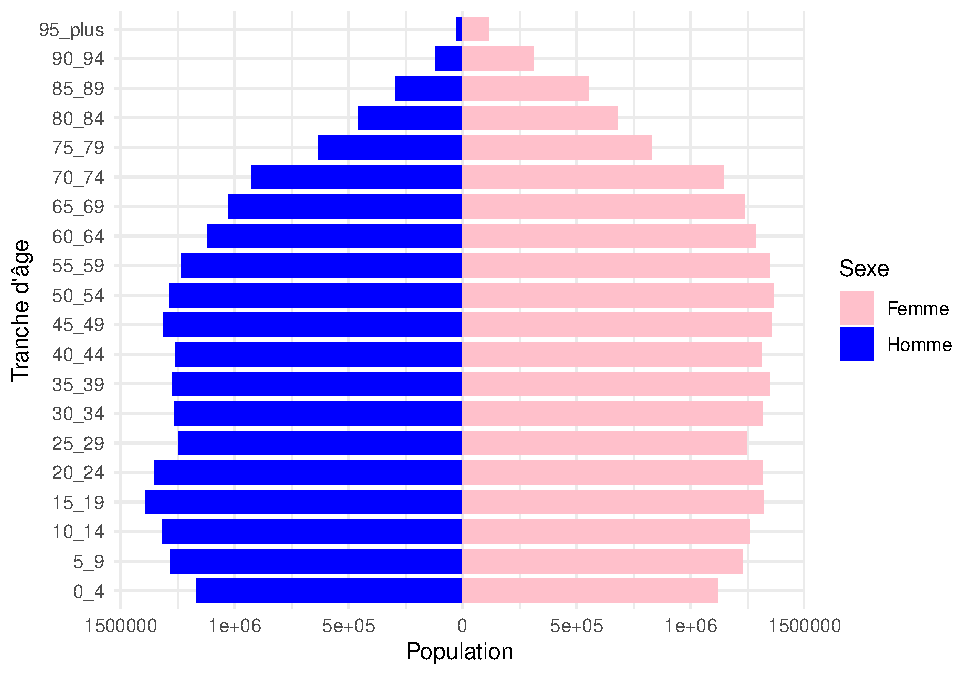
\includegraphics{4_Analyse_Descriptive_files/figure-latex/unnamed-chunk-3-1} 

}

\caption{Pyramide des âges}\label{fig:unnamed-chunk-3}
\end{figure}

\subsubsection{Taux de natalité et taux de
mortalité}\label{taux-de-natalituxe9-et-taux-de-mortalituxe9}

Dans les commmunes étudiées, le taux de natalité et de mortalité sont un
peu élevées avec la plupart des taux variant entre 5 et 15 pour 1000 en
ce qui concerne la natalité et 0 et 20 pour 1000 pour la mortalité. On
remarque une corrélation négative entre ces deux taux. Néanmoins cette
corrélation n'a à priori aucun sens. Par ailleurs, l'observation des
distributions permet de constater que la natalité est de façon générale
élevée par rapport à la mortalité dans les communes étudiées.

\begin{figure}

{\centering 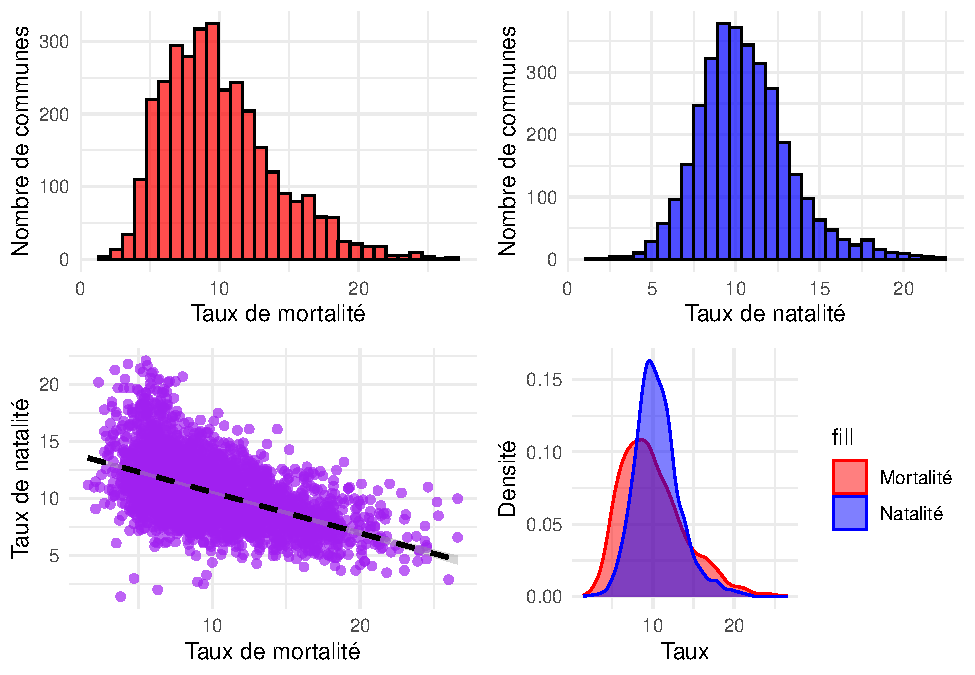
\includegraphics{4_Analyse_Descriptive_files/figure-latex/unnamed-chunk-4-1} 

}

\caption{Taux de Natalité et Taux de Mortalité}\label{fig:unnamed-chunk-4}
\end{figure}

En vue de mieux de mieux voir peut être l'effet de la mortalité sur la
natalité, nous allons nous intéresser alors à une analyse de la
corrélation entre les deux taux par groupe d'age. Nous avons considérer
les groupes d'âge suivants : 0-24, 25-44, 45-60, 60 et plus en fonction
des variables disponibles et ausi à partir de l'information sur l'âge
des femmes en âge de procréer qui est de l'ordre de 25-45 et des
personnes âgées dont l'âge est de plus 60 ans. Ne disposant pas du taux
de mortalité dans chaque groupe, alors nous avons dans notre analyse
opté plutôt pour le pourcentage des femmes de chaque groupe en partant
du principe que la natalité est très souvent liée aux femmes et du fait
que nous pouvons analyser une diminution du pourcentage comme étant dû à
une mortalité. Ainsi sur la base de cette nouvelle hypothèse, voici nos
nouveaux résultats.

\begin{figure}

{\centering 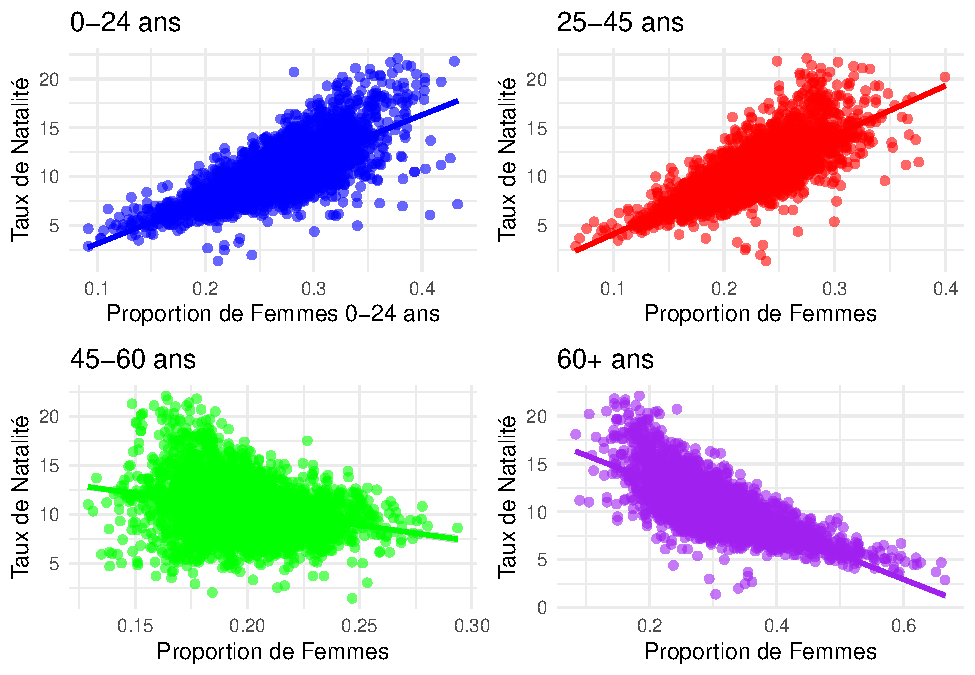
\includegraphics{4_Analyse_Descriptive_files/figure-latex/unnamed-chunk-5-1} 

}

\caption{Taux de Natalité et Pourcentage des femmes dans chaque groupe}\label{fig:unnamed-chunk-5}
\end{figure}

Les résultats nous montrent un lien croissant pour les tranches d'âge
0-24 et 25-45 ans montrant ainsi que dans ces tranches d'âge si le
pourcentage des femmes diminuent (quer l'on pourrait assimiler à une
mort des femmes) alors le taux de natalité diminue. Par ailleurs ceux de
la tranche 45-60 semble n'avoir aucun lien sur le taux de natalité.
Enfin il a été constaté un lien négatif pour la tranche d'âge 60 ans et
plus.

\subsection{Taux et nombre de
consultation}\label{taux-et-nombre-de-consultation}

(Insérer les cartes à ce niveau : Richard doit refaire les cartes et les
insérer)

L'analyse des statistiques descriptives sur le nombre de consultations
annuelles de médecin généraliste entre 2018 et 2022 révèle une
distribution fortement asymétrique à droite, avec une grande dispersion
des données. La moyenne de 19130 consultations, nettement supérieure à
la médiane de 9127, indique la présence de valeurs extrêmes tirant la
distribution vers le haut. Cette asymétrie est confirmée par l'écart
considérable entre le minimum de 1037 et le maximum de 765833
consultations par an.

\begin{figure}

{\centering 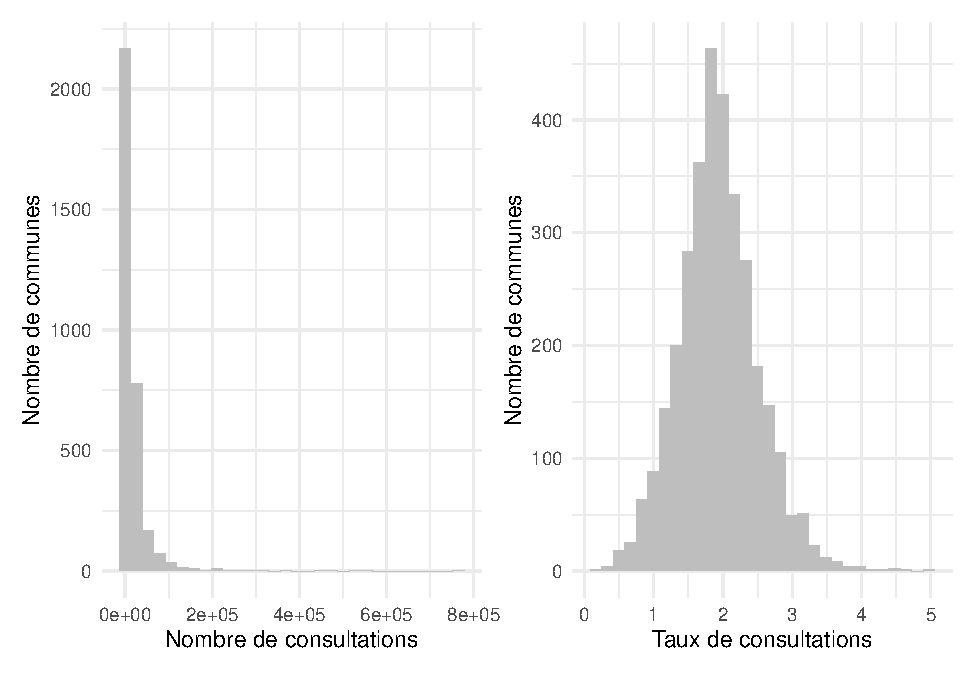
\includegraphics{4_Analyse_Descriptive_files/figure-latex/unnamed-chunk-6-1} 

}

\caption{Distributiion du nombre et du taux de consultations}\label{fig:unnamed-chunk-6}
\end{figure}

La moitié des médecins généralistes effectuent entre 5993 et 17290
consultations annuellement, ce qui suggère une variabilité importante
dans la charge de travail. La médiane de 9127 consultations par an,
équivalant à environ 25 consultations par jour ouvrable, semble plus
représentative de l'activité typique d'un médecin généraliste que la
moyenne influencée par les valeurs extrêmes. Ces statistiques mettent en
lumière la diversité des pratiques et des charges de travail parmi les
médecins généralistes, avec potentiellement quelques cas atypiques
présentant un volume de consultations exceptionnellement élevé.

Le nombre de visites pouvant potentiellement être influencé par la
taille de la commune et donc par sa population, nous avons éliminer cet
effet en calculant le taux de consultations qui n'est autre que le
nombre de consultations moyennes par personnes.

\begin{table}[H]
\centering
\caption{\label{tab:unnamed-chunk-7}Résumé statistique du nombre de visites}
\centering
\begin{tabular}[t]{rrrrrr}
\toprule
Min. & 1st Qu. & Median & Mean & 3rd Qu. & Max.\\
\midrule
\cellcolor{gray!10}{1037} & \cellcolor{gray!10}{5993} & \cellcolor{gray!10}{9127} & \cellcolor{gray!10}{19129.63} & \cellcolor{gray!10}{17290} & \cellcolor{gray!10}{765833}\\
\bottomrule
\end{tabular}
\end{table}

\subsection{Taux de consultation et quelques variables démographiques et
socio-économiques}\label{taux-de-consultation-et-quelques-variables-duxe9mographiques-et-socio-uxe9conomiques}

Nous allons ici, voir s'il y a un lien à priori entre le taux de
consultation et certaines de nos variables explicatives. Ainsi, nous
avons d'abord réalisé une analyse descriptive bivariée puis nous avons
calculé la corrélation de Pearson pour évaluer le lien linéaire entre le
taux de consulation et des variables telles que la population totale, la
part des personnes agées (75 ans et plus), la part de quelques CSP
(ouvriers et retraités).

\subsubsection{Taux de consultation et population
totale}\label{taux-de-consultation-et-population-totale}

En divisant les communes en trois groupes égaux (ou presque égaux) en
fonction de la population totale, il ressort un lien clair entre la
taille des communes françaises et le taux de consultations médicales,
mettant en évidence une tendance où les grandes communes (\textgreater{}
8974 habitants) affichent un taux moyen de consultations supérieur
(1,526810) par rapport aux communes moyennes (1,456356) et petites
(1,383861). Cette observation suggère que l'accès facilité aux
infrastructures médicales dans les zones urbaines contribue à une
utilisation accrue des services de santé. En revanche, les petites
communes, probablement plus isolées et moins dotées en praticiens,
semblent rencontrer des barrières structurelles limitant la fréquence
des consultations.

\begin{table}[H]
\centering
\caption{\label{tab:unnamed-chunk-8}Taux de consultations selon la taille de la commune}
\centering
\begin{tabular}[t]{lr}
\toprule
taille\_commune & Taux de consulations\\
\midrule
\cellcolor{gray!10}{Grande (> 8974)} & \cellcolor{gray!10}{1.526810}\\
Moyenne (4849 - 8974) & 1.456356\\
\cellcolor{gray!10}{Petite (<= 4848)} & \cellcolor{gray!10}{1.383861}\\
\bottomrule
\end{tabular}
\end{table}

\subsubsection{Taux de consultation et population
âgée}\label{taux-de-consultation-et-population-uxe2guxe9e}

L'analyse met en évidence que les communes françaises avec une
population âgée significative (population âgée de 75 ans et plus est
supérieure à la médiane soit plus de 670 habitants âgés de 75 ans et
plus) présentent un taux moyen de consultations inférieur (1,410213)
comparé aux communes où la population âgée est moindre (1,501111). Cette
observation peut refléter des défis spécifiques aux populations plus
âgées, tels que des obstacles physiques ou logistiques pour accéder aux
soins médicaux, ou encore une moindre propension à consulter
régulièrement en raison d'habitudes ou de conditions de santé
chroniques. Ces résultats soulignent un paradoxe apparent, car les
besoins en soins médicaux des personnes âgées sont en général plus
importants, ce qui pourrait indiquer une inadéquation entre l'offre
médicale et les besoins spécifiques de cette tranche d'âge. Cela met en
lumière un enjeu crucial pour les politiques de santé visant à améliorer
l'accès et l'utilisation des services médicaux pour les populations
vieillissantes.

\begin{table}[H]
\centering
\caption{\label{tab:unnamed-chunk-9}Taux de consultations selon la population âgée}
\centering
\begin{tabular}[t]{lr}
\toprule
population\_agee\_importante & consultations\_moyennes\\
\midrule
\cellcolor{gray!10}{Non (<= 670)} & \cellcolor{gray!10}{1.501111}\\
Oui (> 670) & 1.410213\\
\bottomrule
\end{tabular}
\end{table}

\subsubsection{Taux de consultation et
CSP}\label{taux-de-consultation-et-csp}

Aucune catégorie ne semble montrer une relation linéaire évidente avec
le taux de visite. Par ailleurs, pour toutes les catégories
socio-professionnelles, la majorité des communes se situent dans une
plage de proportions faibles, ce qui limite la variabilité observable
dans les relations. Une analyse statistique supplémentaire, comme le
calcul de corrélations, serait nécessaire pour confirmer ou infirmer les
relations observées visuellement.

\begin{figure}

{\centering 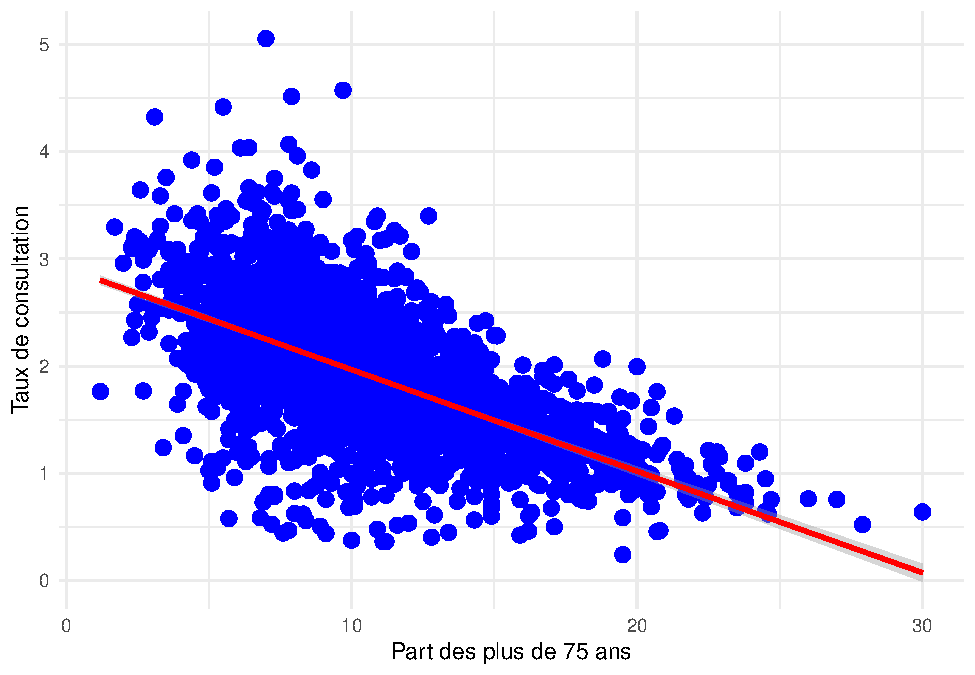
\includegraphics{4_Analyse_Descriptive_files/figure-latex/unnamed-chunk-10-1} 

}

\caption{Relations entre le taux de consultatiosn et certaines catégories socioprofessionnelle}\label{fig:unnamed-chunk-10-1}
\end{figure}
\begin{figure}

{\centering 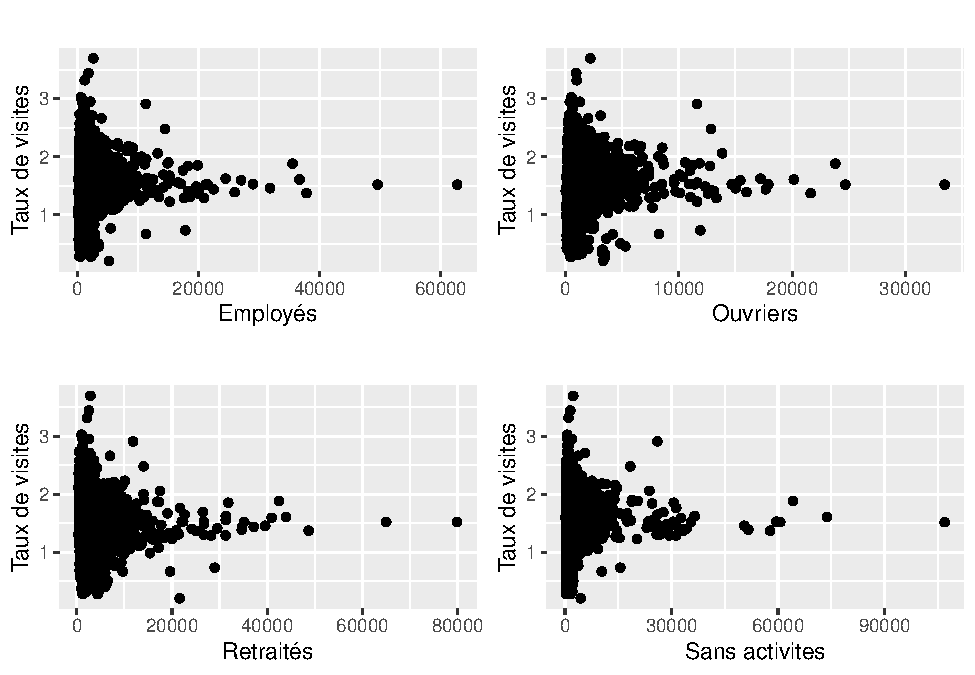
\includegraphics{4_Analyse_Descriptive_files/figure-latex/unnamed-chunk-10-2} 

}

\caption{Relations entre le taux de consultatiosn et certaines catégories socioprofessionnelle}\label{fig:unnamed-chunk-10-2}
\end{figure}

(Trouver un titre pour cette section et analyser : Alex)

\begin{figure}

{\centering 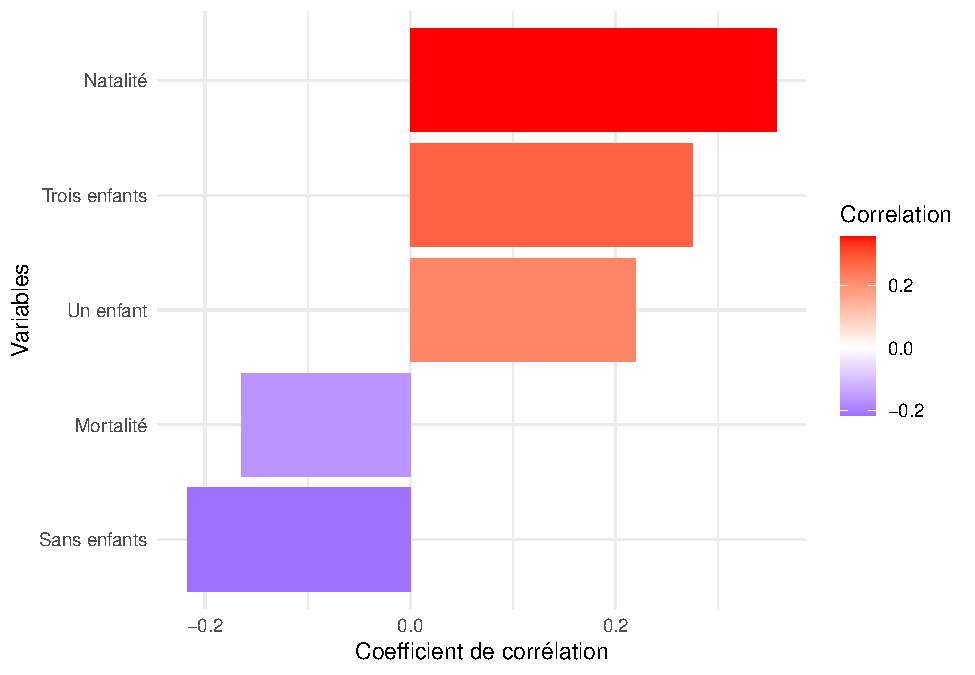
\includegraphics{4_Analyse_Descriptive_files/figure-latex/unnamed-chunk-11-1} 

}

\caption{Corrélations entre le nombre de visite et quelques variables}\label{fig:unnamed-chunk-11}
\end{figure}

\subsection{Analyse spatiale}\label{analyse-spatiale}

Après une analyse de nos données en ne tenant pas compte de l'effet
spatial, nous allons à présent poursuivre avec une analyse qui tient
compte de celui-ci. Nous allons ici faire une analyse basée sur le
diagramme de Moran. Le diagramme de Moran permet d'analyser la structure
spatiale du taux de consultations. Il est constitué d'un nuage de points
où l'axe des abscisses représente les valeurs centrées du taux de
consultations (\(yy\)), et l'axe des ordonnées montre les valeurs
moyennes du taux de consultations pour les zones voisines (\(Wyy\)),
avec \(W\) étant la matrice de poids normalisée. En raison de la
centration de \(yy\) et de la normalisation de \(W\), la moyenne
empirique de \(Wyy\) est égale à zéro.

Le diagramme inclut aussi une droite de régression linéaire entre
\(Wyy\) et \(yy\), ainsi que les lignes \(y=0\) et \(Wyy=0\), qui
divisent l'espace en quatre quadrants.

\begin{itemize}
\tightlist
\item
  \textbf{Quadrant 1 (haut à droite)} : Les zones avec un taux de
  consultations plus élevé que la moyenne, entourées de zones présentant
  également un taux de consultations élevé (autocorrélation spatiale
  positive, structure \textbf{high-high}).
\item
  \textbf{Quadrant 3 (bas à gauche)} : Les zones avec un taux de
  consultations plus faible que la moyenne, entourées de zones
  présentant un taux de consultations également faible (autocorrélation
  spatiale positive, structure \textbf{low-low}).
\item
  \textbf{Quadrant 2 (bas à droite)} : Les zones avec un taux de
  consultations plus élevé que la moyenne, mais entourées de zones
  présentant un taux de consultations plus faible (autocorrélation
  spatiale négative, structure \textbf{high-low}).
\item
  \textbf{Quadrant 4 (haut à gauche)} : Les zones avec un taux de
  consultations plus faible que la moyenne, mais entourées de zones avec
  un taux de consultations plus élevé (autocorrélation spatiale
  négative, structure \textbf{low-high}).
\end{itemize}

La densité des points dans chaque quadrant permet de visualiser la
structure spatiale dominante du taux de consultations. Ce diagramme aide
aussi à identifier les zones atypiques, qui ne suivent pas la structure
spatiale générale, facilitant ainsi l'analyse des résultats que vous
obtiendrez par la suite. Vu le noimbre de nos communes la mise sur le
graphique des noms de toutes les communes allaient être compliqué. POur
cela, nous avons choisi au hasard 4 communes par cadrants. Ainsi, Ce
diagramme de Moran illustre la corrélation spatiale des taux de
consultation par commune et ceux des communes voisines. La tendance
générale, représentée par la droite de régression rouge, montre une
relation positive entre ces taux, confirmant ainsi une autocorrélation
spatiale. Autrement dit, les communes ayant un taux élevé de
consultations ont tendance à être entourées par d'autres communes avec
un taux similaire, et inversement.

Dans le quadrant HH (Haut-Haut), représenté en rouge, on retrouve des
communes comme Saint-Saulve, Le Bouscat et Bruay-la-Buissière. Celles-ci
affichent un taux de consultation élevé et sont entourées par des
communes présentant également des taux élevés. Cela indique une
concentration géographique des consultations médicales, qui peut
s'expliquer par une offre de soins plus développée ou une demande locale
particulièrement forte.

Le quadrant HL (Haut-Bas), en violet, comprend des communes comme
Saint-Jacques-de-la-Lande et Le Portel. Ces communes ont un taux élevé
de consultations, mais sont entourées de communes où les taux sont plus
faibles. Ce contraste peut suggérer que ces villes disposent d'une offre
de soins plus attractive que leurs voisines, attirant ainsi des patients
des alentours.

À l'inverse, dans le quadrant LH (Bas-Haut), en vert, on trouve des
communes comme Aix-en-Provence, Ribécourt-Dreslincourt et L'Isle-Adam.
Ces communes affichent un faible taux de consultation, tandis que leurs
voisines présentent des taux plus élevés. Ce phénomène peut s'expliquer
par le fait que les habitants de ces villes se rendent dans les communes
avoisinantes pour leurs consultations, soit en raison d'un manque
d'infrastructures médicales locales, soit par préférence pour des
services situés ailleurs.

Enfin, le quadrant LL (Bas-Bas), en orange, inclut des communes comme
Saint-Jean-le-Blanc, Romorantin-Lanthenay et Le Breuil. Ces villes ont
un faible taux de consultation et sont entourées de communes où les taux
sont également bas. Cela peut indiquer une accessibilité réduite aux
soins de santé, une moindre densité médicale, ou encore une faible
demande locale pour des consultations.

En résumé, cette analyse met en évidence des disparités territoriales
dans la répartition des consultations médicales. Certaines communes
concentrent les services et attirent les patients des alentours, tandis
que d'autres souffrent d'un accès limité aux soins, renforçant ainsi les
inégalités spatiales en matière de santé.

\begin{figure}

{\centering 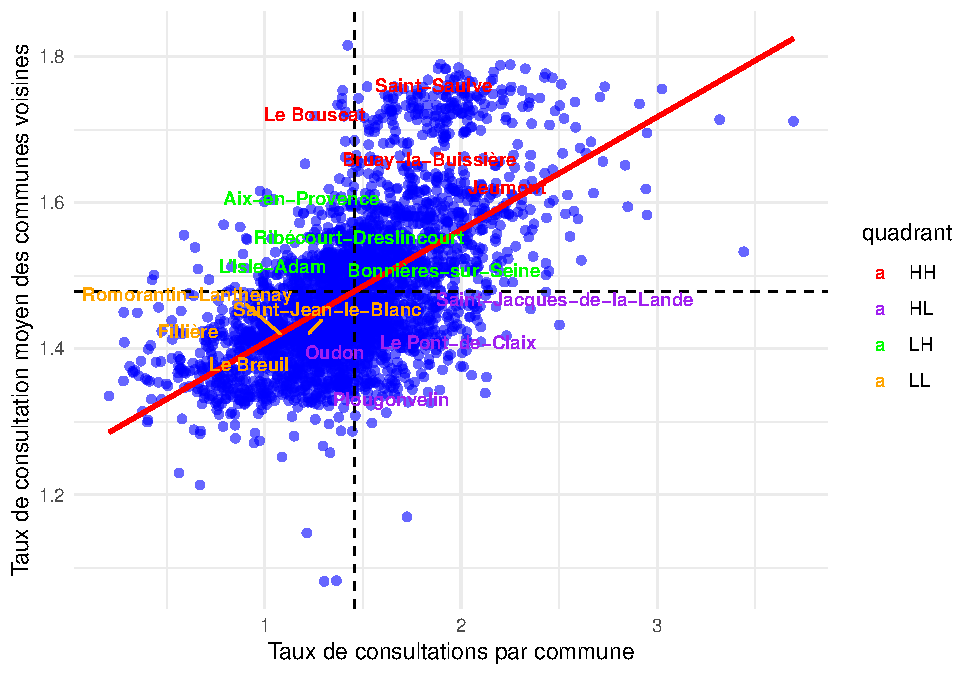
\includegraphics{4_Analyse_Descriptive_files/figure-latex/unnamed-chunk-21-1} 

}

\caption{Moran Plot avec visibilités de quelques communes}\label{fig:unnamed-chunk-21}
\end{figure}

\subsubsection{Autocorélation Locale}\label{autocoruxe9lation-locale}

\begin{figure}

{\centering 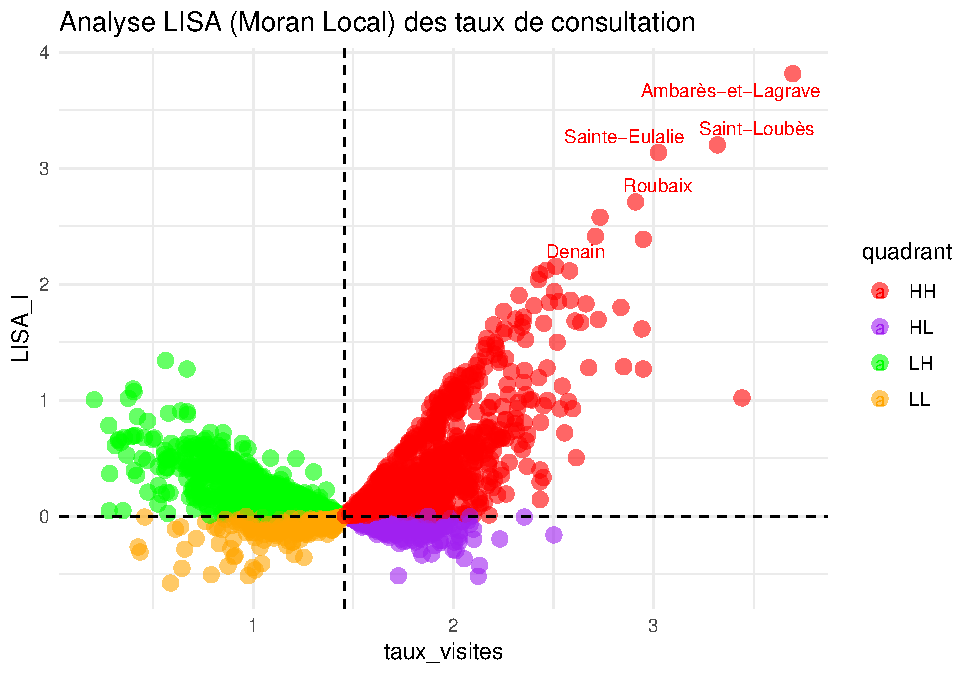
\includegraphics{4_Analyse_Descriptive_files/figure-latex/unnamed-chunk-22-1} 

}

\caption{Clusters sur la base du LISA}\label{fig:unnamed-chunk-22}
\end{figure}

En se basant sur l'analyse par cluster fourni pour le LISA (local
Indicator or Spatial Association), nous pouvons remarquer que le cluster
HH est celui regroupant le plus de communes suivi du cluster LH. Ceci
dit une grande partie des communes ont des taux élevées et entourées par
des communes de taux élevées ou encore des taux bas et entourées par des
communes de taux élevées.

\end{document}


%\input{5_Modelisation}

%\input{6_Discussion}

%\input{7_Conclusion}

\bibliographystyle{plain}

\bibliography{references}


\section*{ANNEXES}\addcontentsline{toc}{section}{ANNEXES}

\begin{figure}
    \centering
    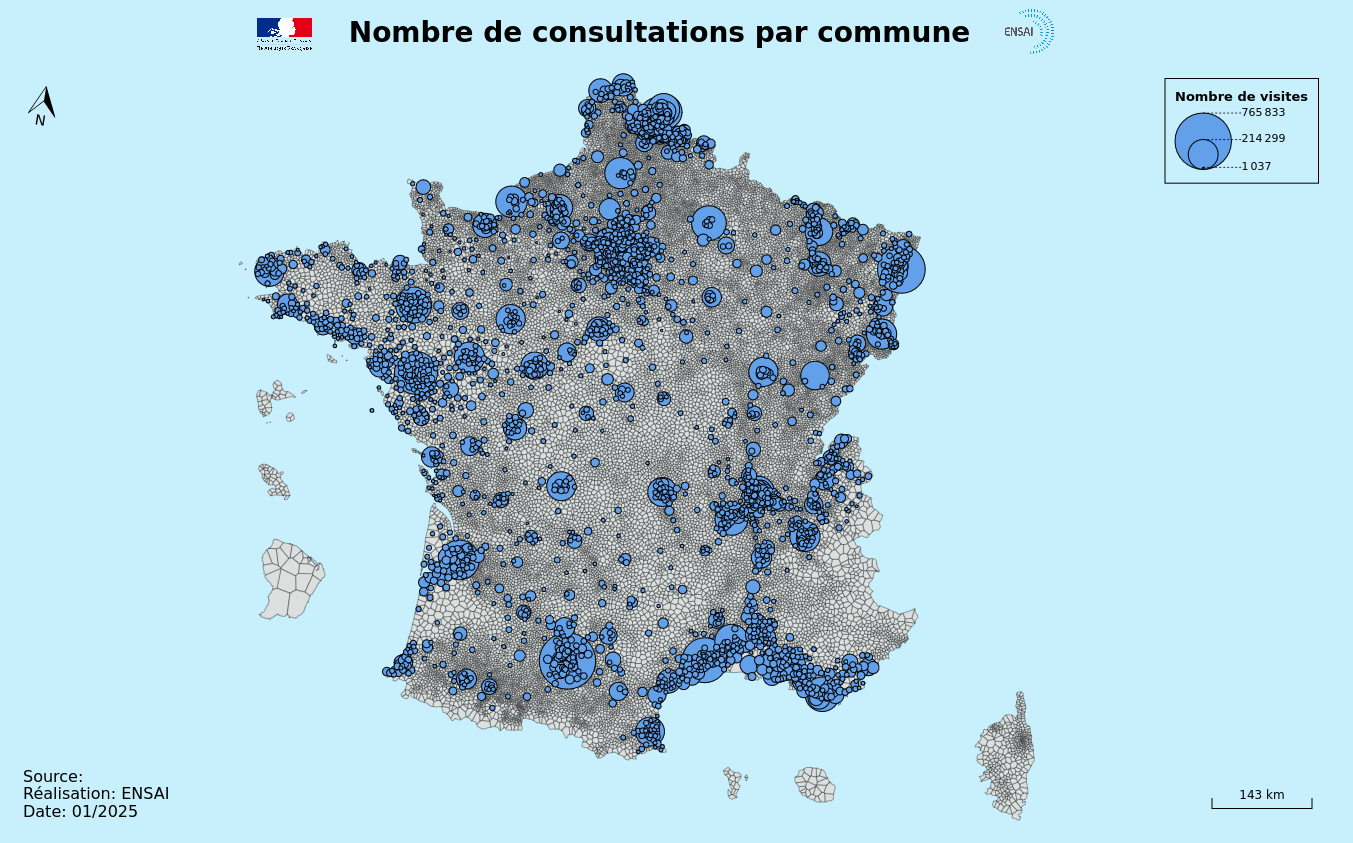
\includegraphics[width=1\linewidth]{../cartes/nombre_de_consulatations}
    \caption{Carte du nombre de consultations par commune}
    \label{fig:figure}
\end{figure}
\begin{figure}
    \centering
    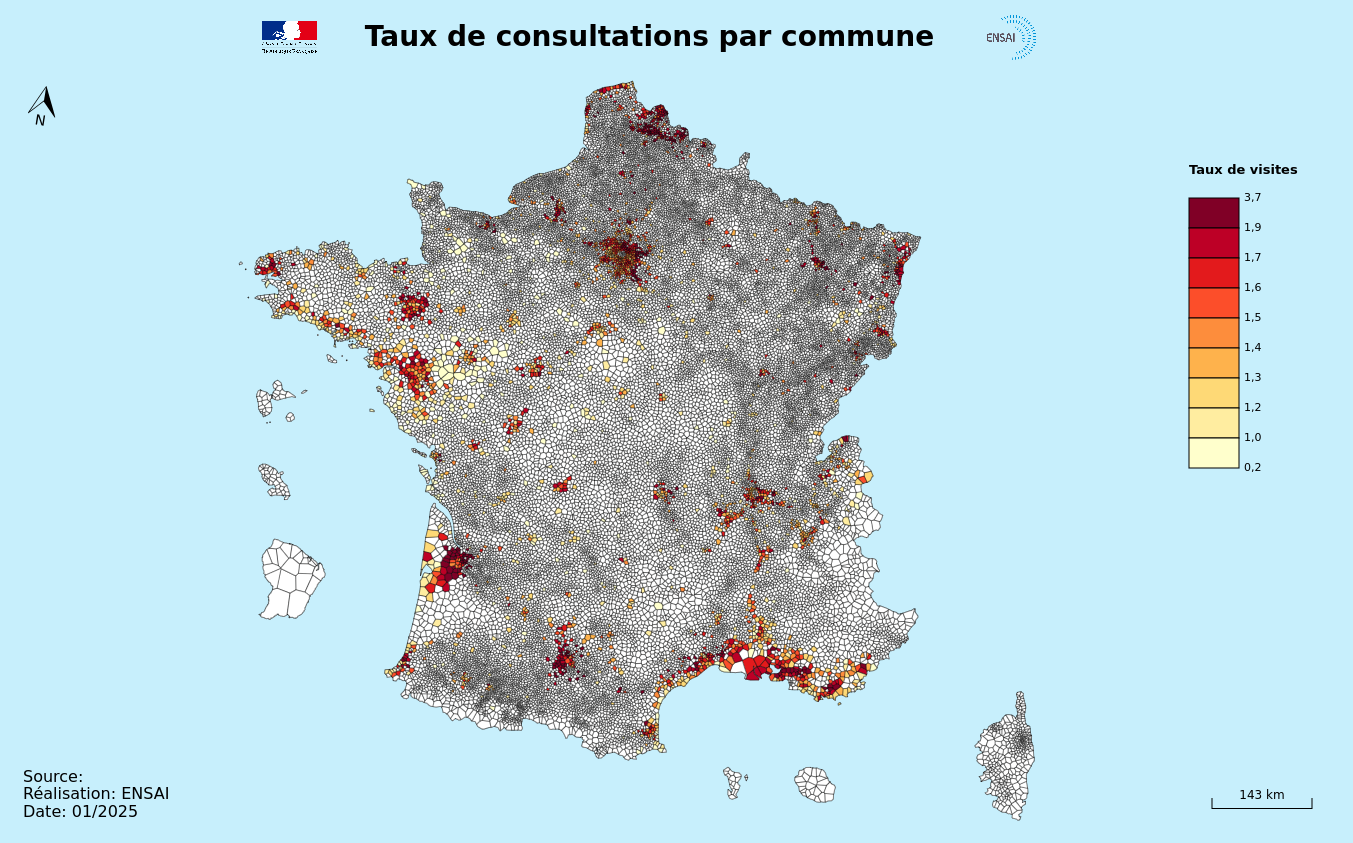
\includegraphics[width=1\linewidth]{../cartes/taux_de_consultations}
    \caption{Carte du taux de consultations par commune}
    \label{fig:figure}
\end{figure}
\begin{figure}
    \centering
    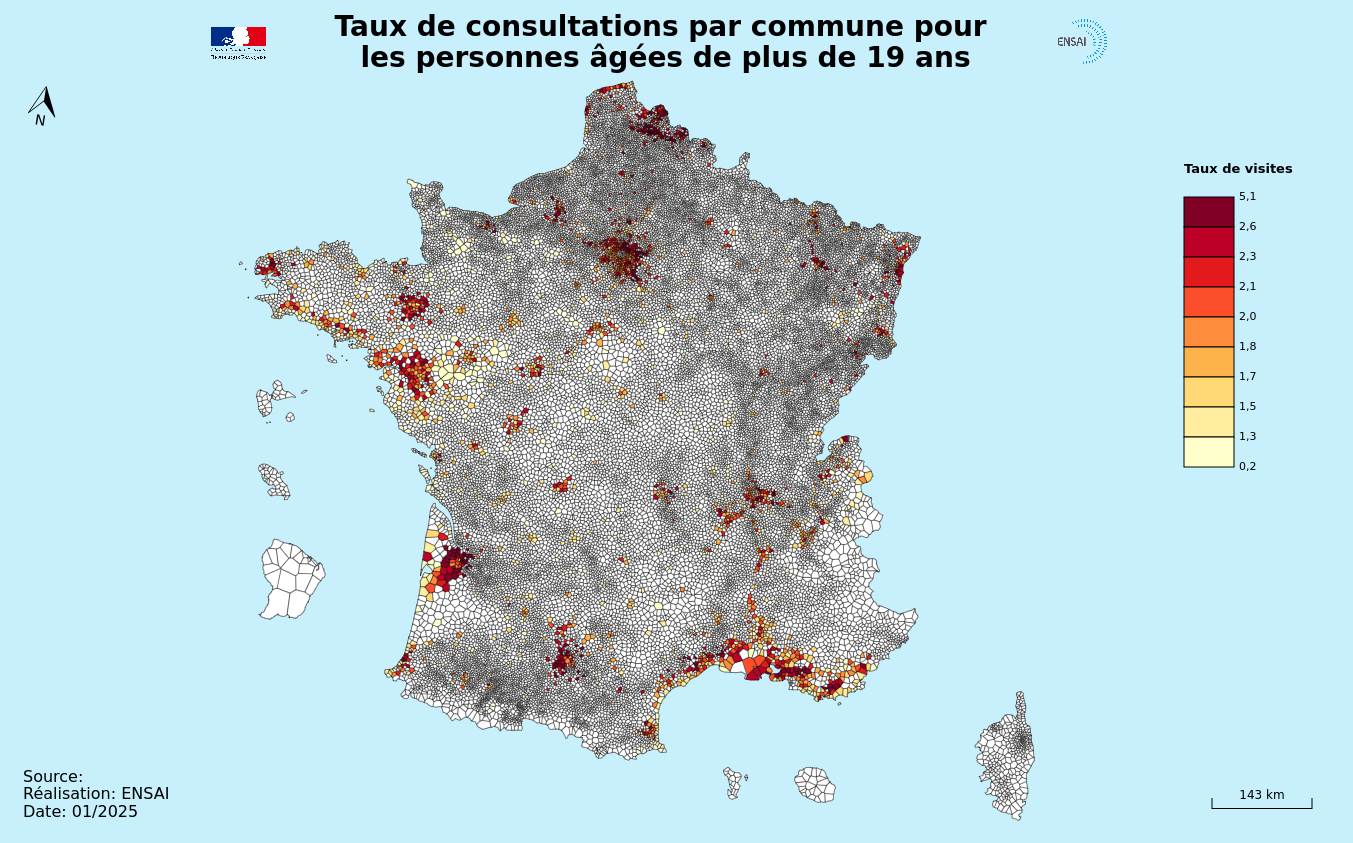
\includegraphics[width=1\linewidth]{../cartes/taux_de_consultations_plus_19_ans}
    \caption{Carte du taux de consultations par commune pour les plus de 19 ans}
    \label{fig:figure}
\end{figure}




\end{document}
